\begin{figure}[H]
	\centering
	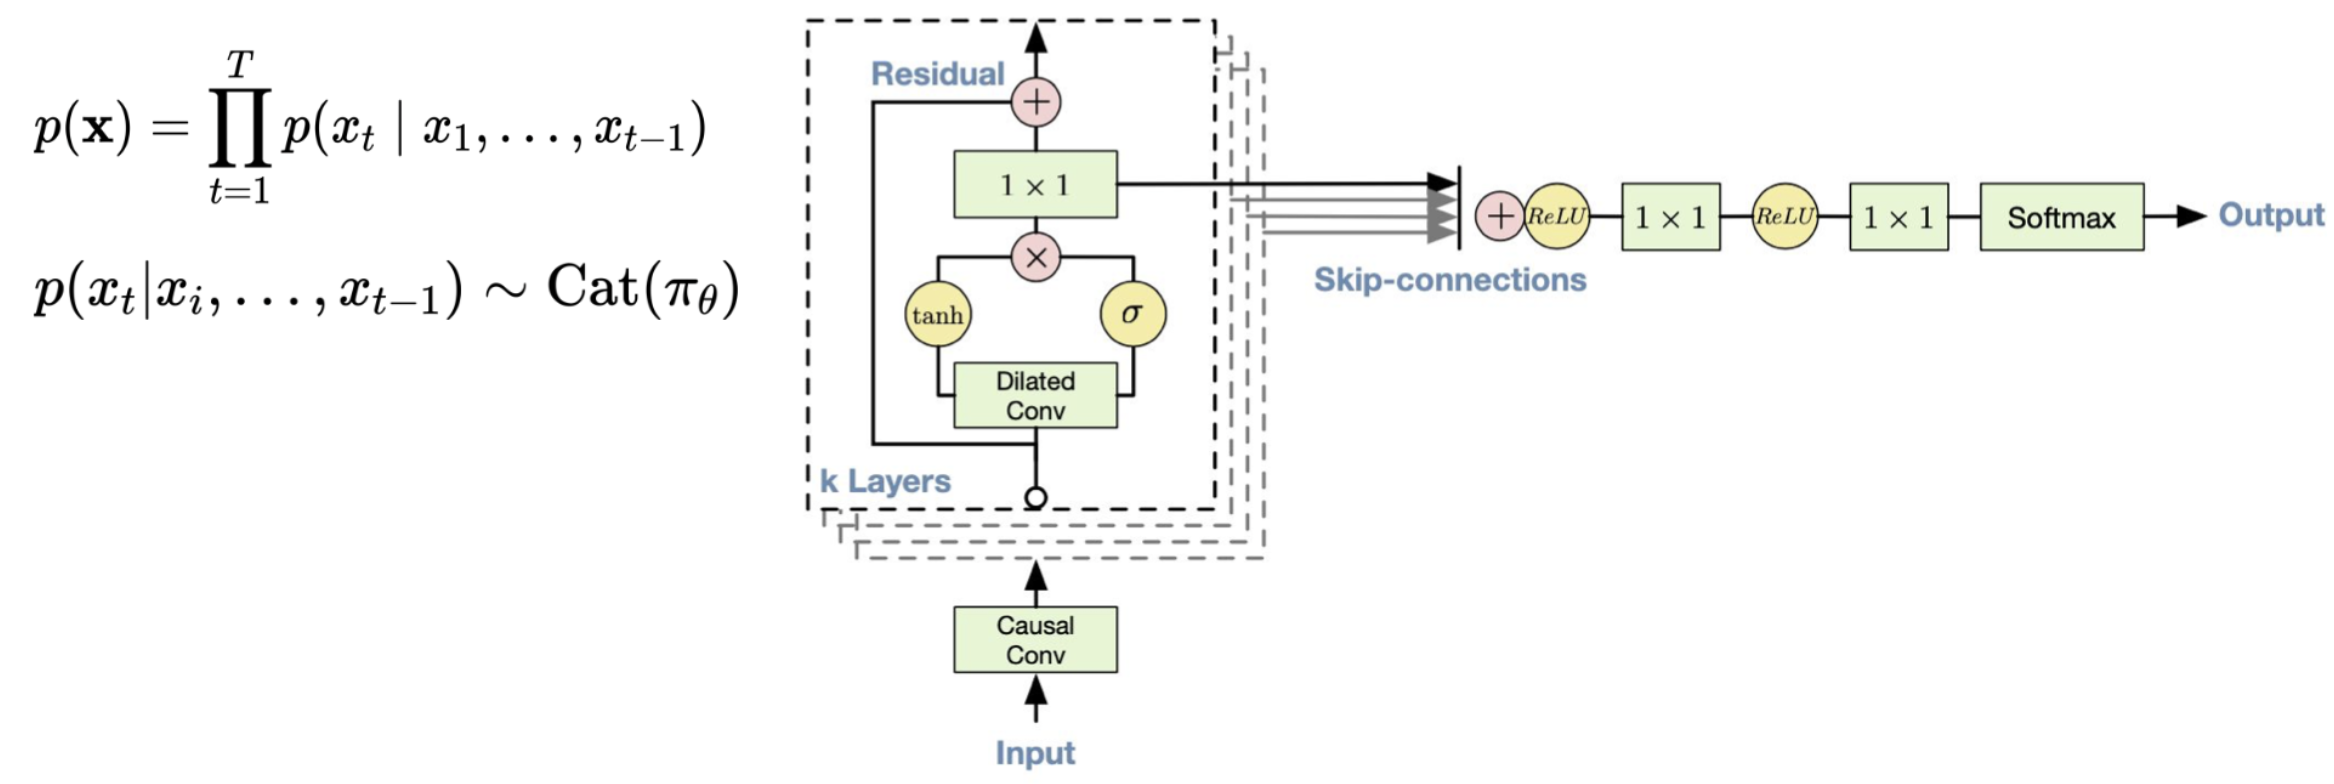
\includegraphics[width=\linewidth]{13_2.png}
	\label{fig:13_2}
\end{figure}


Авторегрессионная модель (моделируем условные вероятности по всем предыдущим сэмплам). Вход -- амплитуды, в train, например, 100 ground truth сэмплов. Для них у нас, например, 12 мелов. Прогоняем через каузальную свертку мелы, растягивая их. Берем первые 99 сэмплов и загоняем в нашу модель. Для каждого сэмпла предсказываем следующий со сдвигом 1. По такой же схеме в строительном блоке (ниже) обуславливаем сэмплы на мелы. Когда будем считать ошибку, возьмем последние 99 сэмплов. Амплитуды проходят через k одинаковых строительных блоков. 


Структура блока:

\begin{figure}[H]
	\centering
	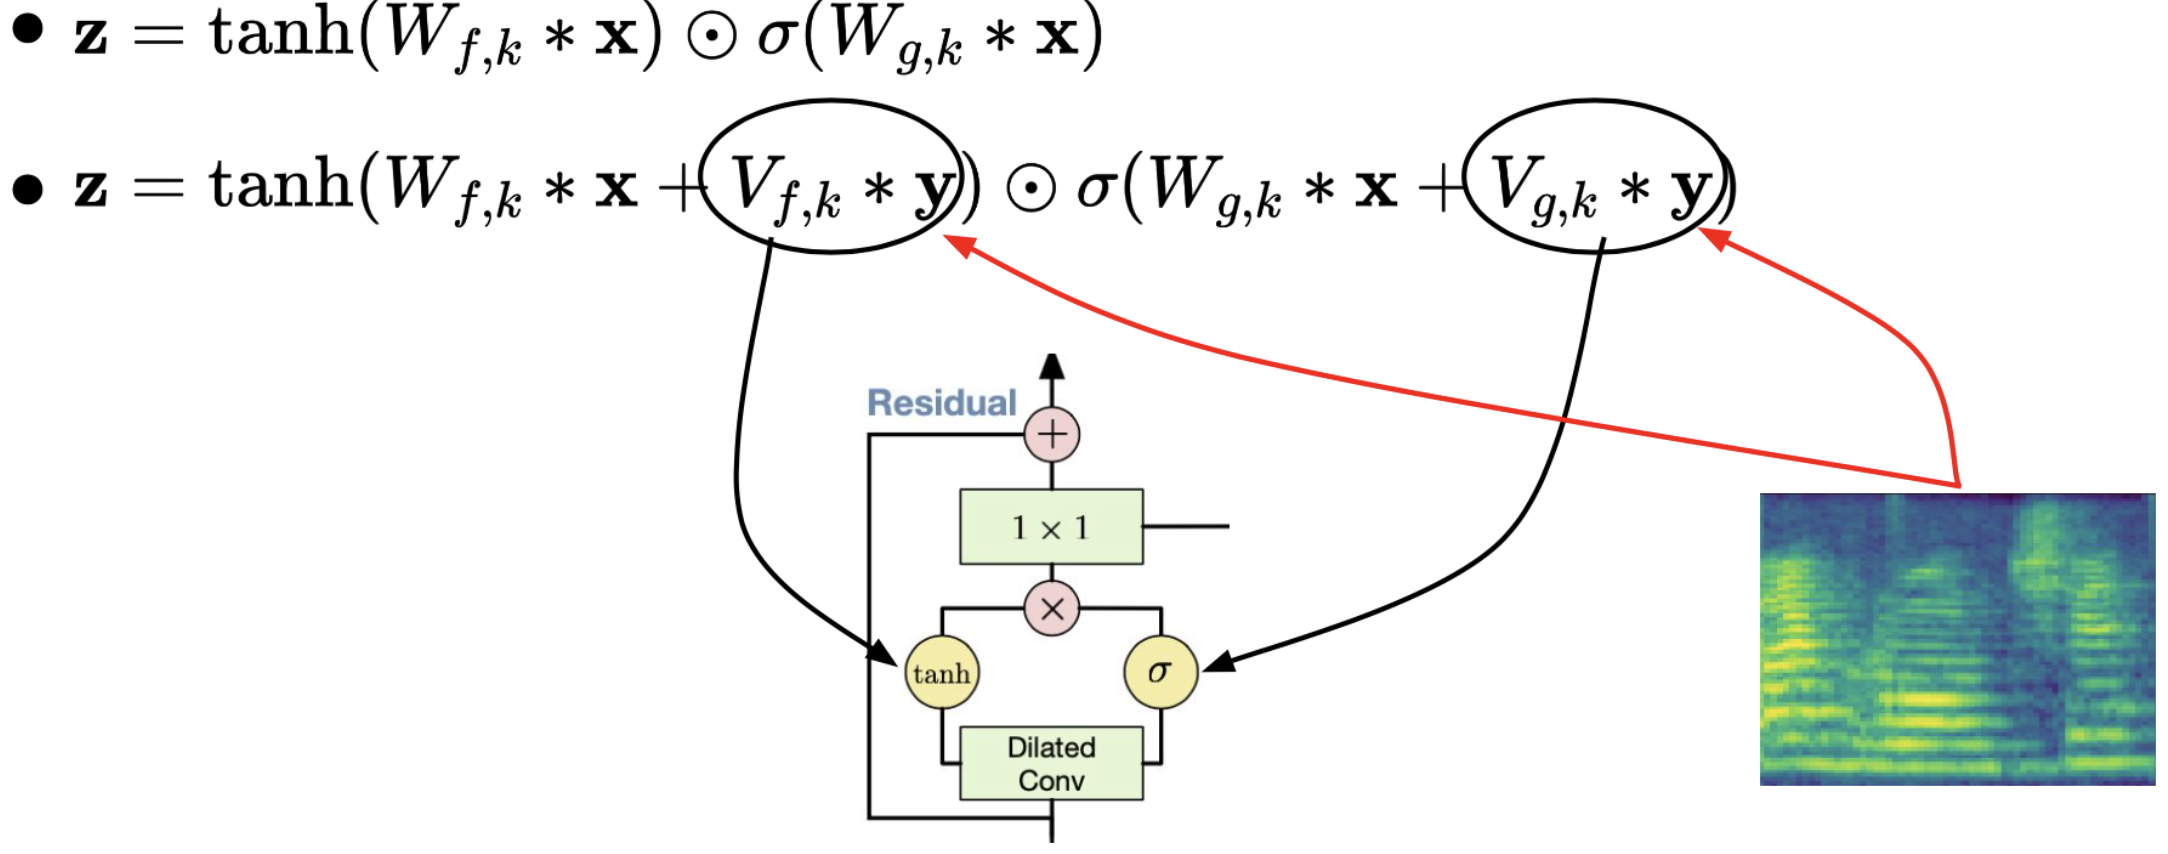
\includegraphics[width=\linewidth]{13_1.png}
	\label{fig:13_1}
\end{figure}



\begin{enumerate}
    \item Каждый сигнал x (на схеме перед dilated conv) сворачиваем двумя каузальными свертками $W_f$ и $W_g$. На каждую кладем сигмоиду и поэлементно перемножаем. Наша сигмоида выучивает, на какие куски аудио смотреть, на какие -- нет. 1 открывает gate внимания, 0 -- закрывает. 1х1 -- свертка с ядром kernel size. Яичко. Это не так важно.
    
    FYI:
    
    Dilated свертки увеличивают рецептивное поле. Dilation растет экспоненциально -- от 1 до 1000 с шагом 2 в каокй-то степени. Рецептивное поле раздувается, что позволяет нам моделировать очень длинные зависимости. Нам это важно, потому что в wav много занимает, но хранит мало информации. Одна секунда -- 16 000 сэмплов. Секунда -- мало, данных -- много.
    
    Второй момент -- каузальные свёртки. Нужны, чтобы моделировать авторегрессию. На стандартной свертке синий -- первый уровень, серый -- второй уровень. На вход синие данные сворачиваем сверткой размером 3 со страйдом 1. Три шарика свернули в один. На самом центральном шарике видно, что он сворачивается, при этом берет вклад и слева, и справа -- смотрит и в прошлую, и в будущее. Нам это не подходит, так как мы не хотим смотреть в будущее. Нам нужно как-то свертку обрубать. Вклад каждого шарика серого или оранжевого цвета или из настоящего, или из будущего. Как делать? Можно добавлять в саму свёртку паддинг. Левый -- правильный, правый -- лишний. Вырезаем его. Можно маскировать свертки. С паддингами проще читать код. 
    
   
    \item Предсказываем, исходя из mel-синтезиса. Сворачиваем mel с двумя свертками (в формуле y -- mel, V -- свертки). Так мы обуславливаем нашу генерацию. Так считаем каждый слой. x и спектрограмма разного размера по времени, и чтобы они совпадали мы должны растянуть спектрограмму до размера сэмпла. Это делается или transpose сверткой, или линейной интерполяцией.
\end{enumerate}

Skip-connections для каждого сэмпла выдает распределение для следующего.

Дальше MuLaw encoding. У каждого представления 16000 сэмплов, и каждый сэмпл -- число. Один сэмпл занимает 16 бит, $2^{16}$ значений. Чтобы софтмакс на таком количестве не ломался, ужимаем амплитуды с сохранением выразительности (см. вопрос 12).

Функция потерь. У нас должно быть какое-то распределение. Чтобы было категориальное, в самом конце на каждый сэмпл навешиваем softmax и предсказываем вероятность той или иной амплитуды. Но в целом нам ничего не мешает использовать нормальное распределение. Или смесь распределений.

Почему медленно: каузальные свертки. Мы делаем что-то для каждого сэмпла отдельно, т. к. следующий зависит от предыдущего. Усовершенствованные сетки работают с несколькими сэмплами одновременно. Например, изначально кормятся белым шумом:


\begin{figure}[H]
	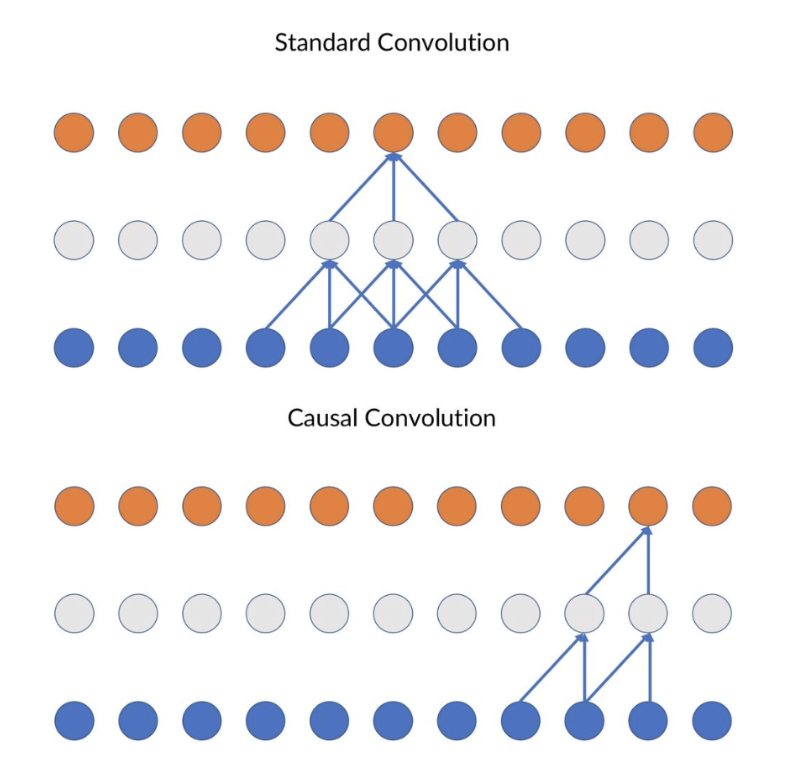
\includegraphics[width=0.5\linewidth]{13_4.png}
	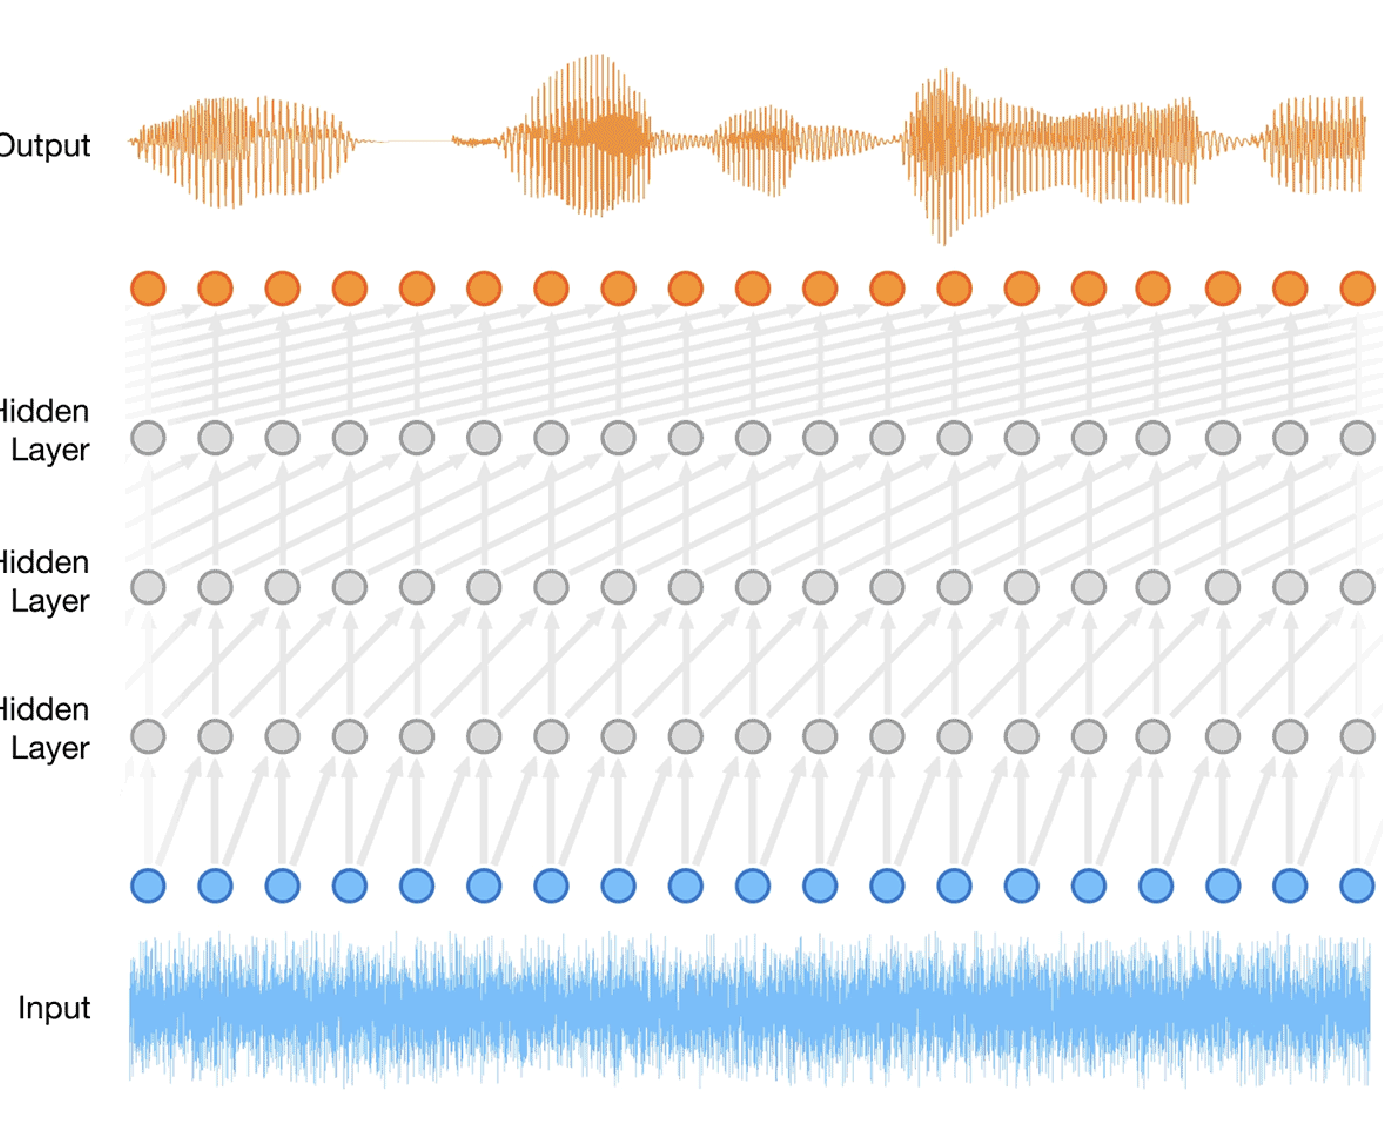
\includegraphics[width=0.5\textwidth]{13_3.png}
	\label{fig:13_3}
\end{figure}
